\subsection{Analysis with Turtles}

 Turtles are the mechanism used to track the flow of API objects around the user code, as described in Section~\ref{sec:example}.  As described there,  the basic approach is that all returns from API calls are represented as instances of a single ``turtle'' type and all calls on such objects return new instances of that type.  Similarly, access to properties of those objects return the object itself.  This can be expressed easily in common analysis frameworks and formalisms, as it requires customization of three aspects of analysis.  We present these three both in terms of the analysis abstractions that need to be customized and also in terms of how this is accomplished in WALA.

\begin{figure}[htb]
\begin{center}
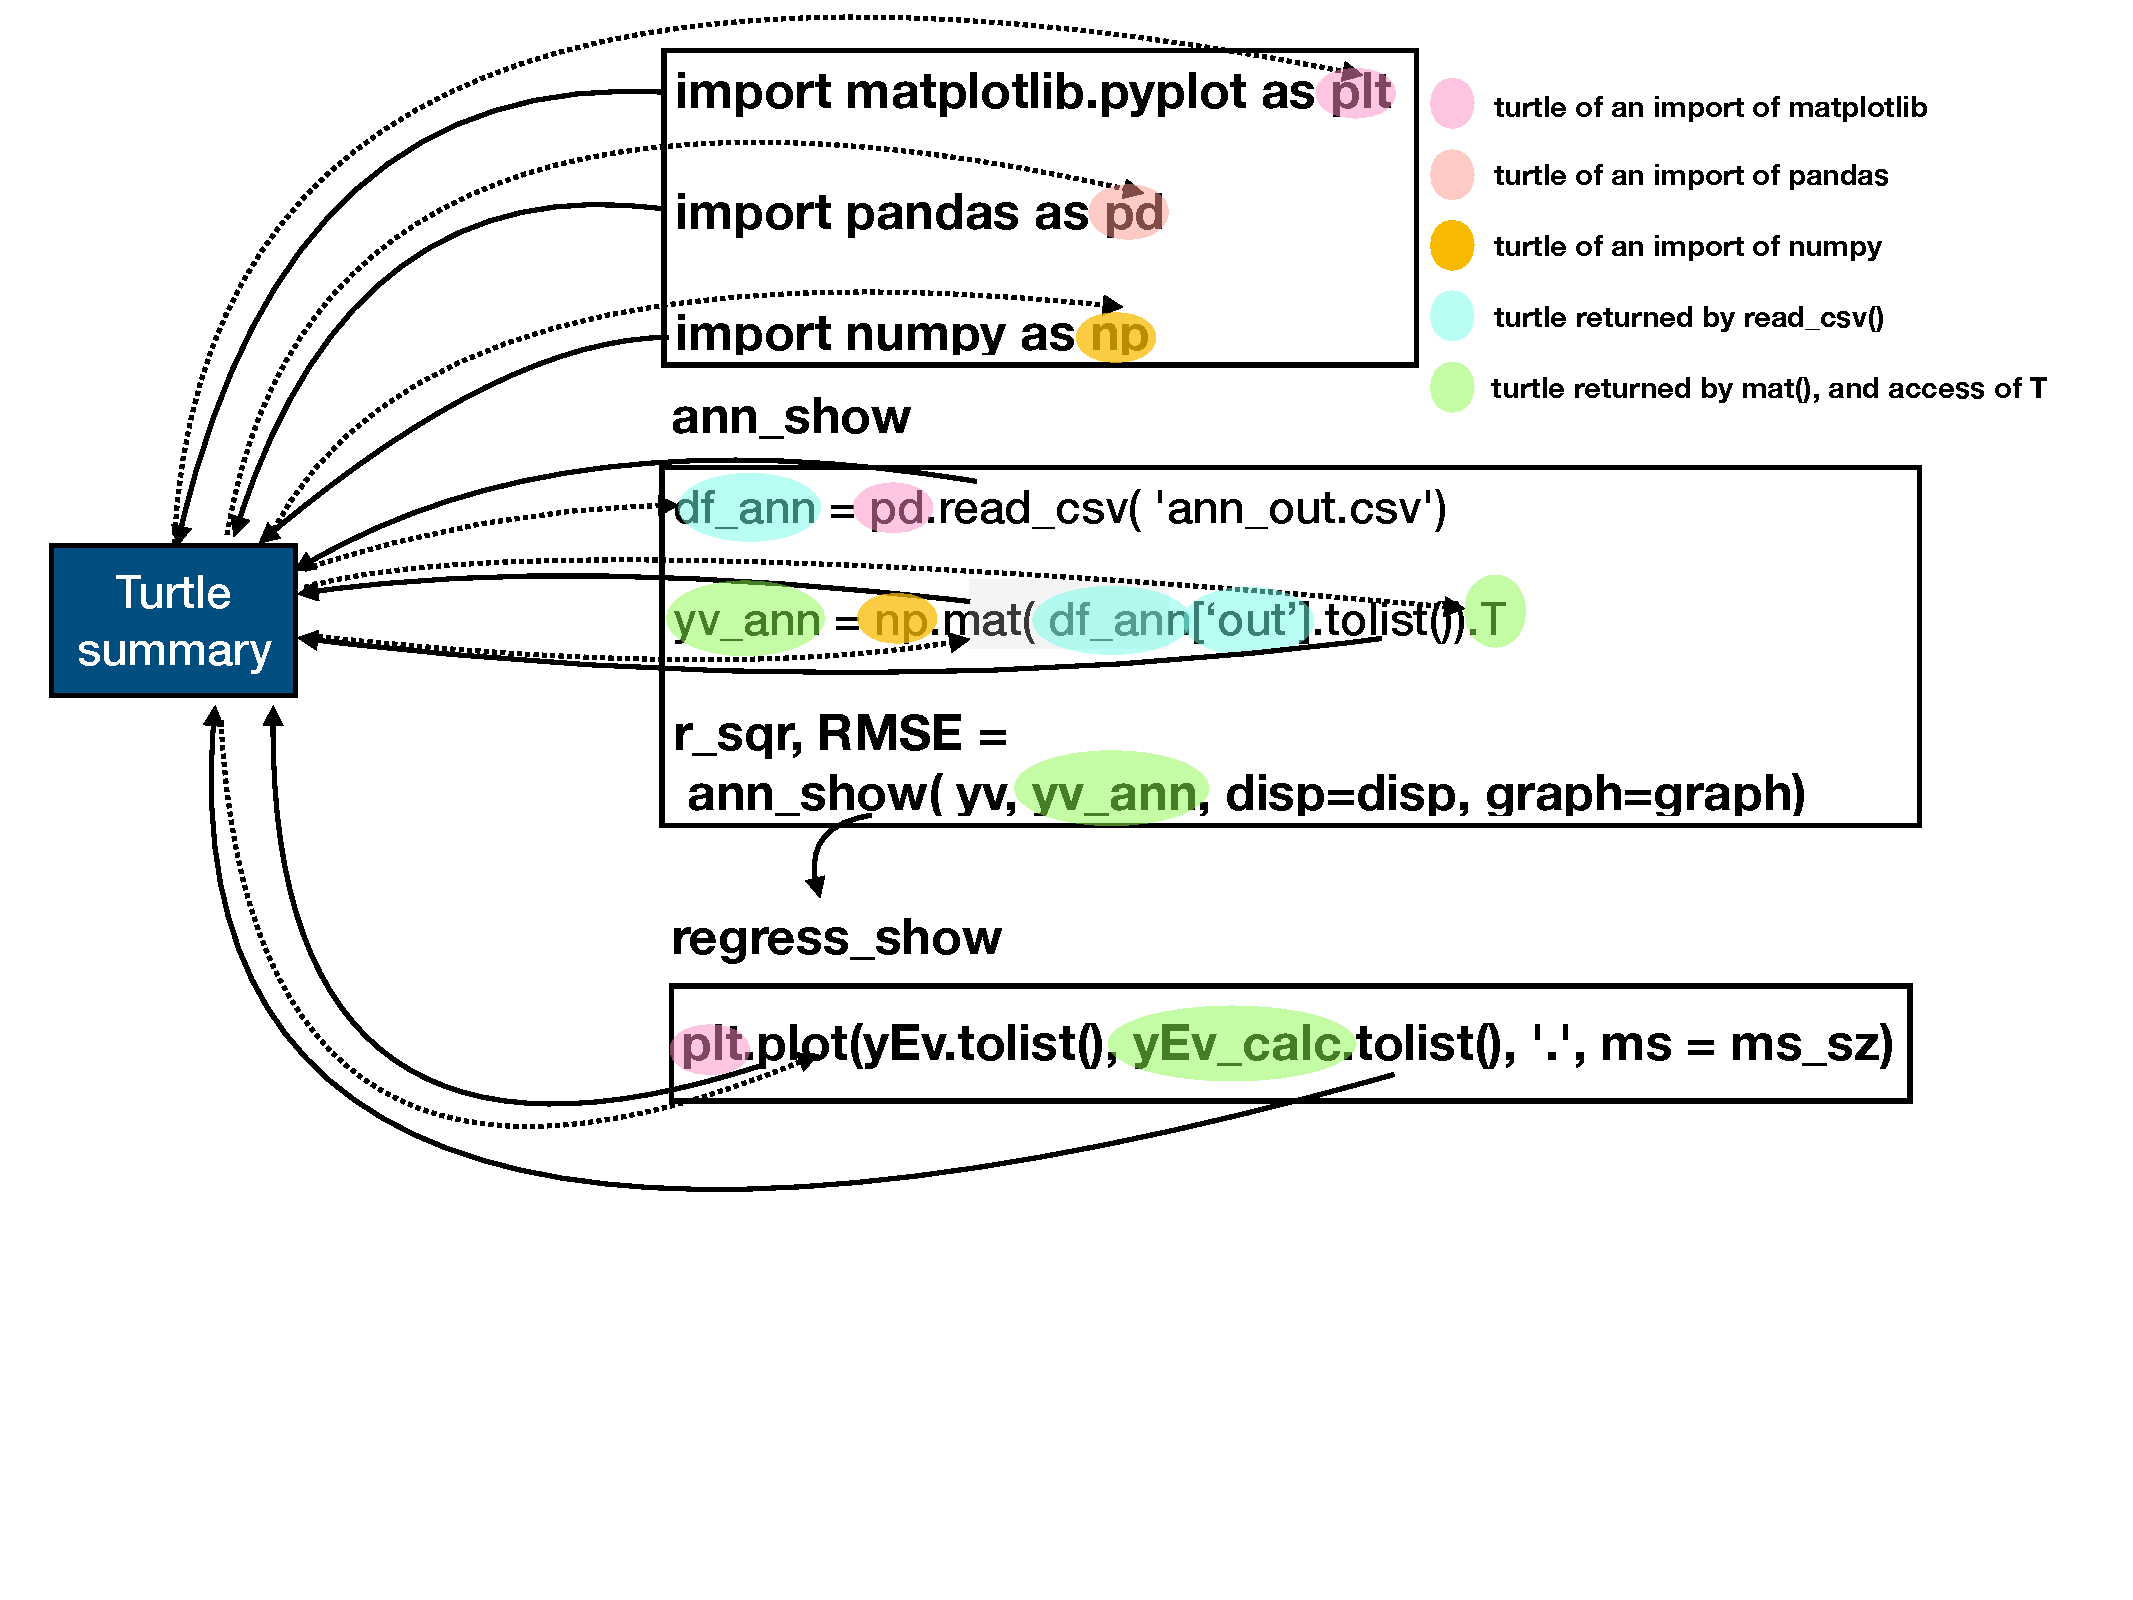
\includegraphics[width=3.5in]{turtle_figure}
\end{center}
\caption{Dataflow of turtles in example code}
\label{fig:dataflow}
\end{figure}

The dataflow induced by our turtle analysis is represented in Figure~\ref{fig:dataflow}.  There is an abstract turtle summary that simply returns new turtles when called.  The {\tt import} statements each are represented as calls to this summary, returning new turtles represented by colors in Figure~\ref{fig:dataflow}.  Calls to {\tt read\_csv}, {\tt mat}, and {\tt to\_list} are calls on turtles themselves, so they also are represented by further calls to the turtle summary.  The access to {\tt df\_ann[out]} is access to the state of a turtle, which is represented by the same turtle, so both values use the same turtle color.
   
\begin{figure*}[htb]
\begin{centering}
\lstinputlisting[language=Python,escapechar=|,numbers=none]{./ir.txt}
\caption{WALA IR of the {\tt ann\_post} function from example code}
\label{code:ann_post}
\end{centering}
\end{figure*}

WALA performs a standard combined call graph construction and pointer analysis that computes, for each call site, what functions may be called, and for each value, what objects it may hold.  Analysis starts at a root function, analyzing each instruction, adding functions found at call sites to a work queue.  To make the workings of the analysis more concrete, we will use the WALA IR for the {\tt ann\_post} function of Figure~\ref{running_example}, shown in Figure~\ref{code:ann_post}.  The code is organized as a sequence of basic blocks (denoted {\tt BB0}, {\tt BB1}, etc) of operations such as property reads, and all values are in Static Single Assignment form.  We show how the analysis work for turtles by stepping through what the analysis does when {\tt ann\_post} is analyzed:
\begin{itemize}
\item instruction 0 reads {\tt pd} from the script itself.  This was imported into the script as shown on line~\ref{line:importpd} of Figure~\ref{running_example}.  This assigns the variable {\tt pd} in the top-level script; {\tt ann\_post} is nested within the script, and this instruction reads the analysis estimate of {\tt pd}, which we'll call turtle $t_1$, from the script and adds it to {\tt v9}. 
\item instruction 1 reads the property {\tt read\_csv} from {\tt v9}.  At this point {\tt v9} holds $t_1$, which is a turtle, so the result is assigning $t_1$ to {\tt v7}.  Instructions called {\tt getfield} and {\tt fieldref} all represent field accesses, and are handled analogously.
\item instruction 2 calls {\tt v7} as a function.  Since {\tt v7} hold $t_1$ and the semantics of function calls on turtles is to create a new turtle, we assign the new turtle $t_2$ to {\tt v6}.
\end{itemize} 
The rest of the instructions are mostly analogous, except two
\begin{itemize}
\item instruction 12 reads a normal Python function from the global variable {\tt ann\_show}, which we denote $f_1$
\item instruction 15 calls $f_1$.  This is not a turtle, so the code for that function is added to the work queue of the analysis.  $v2$ is an argument {\tt yv} passed into the function, $v13$ represents the field read of $T$ that gets assigned to {\tt yv\_ann}, and $disp:3$ and $graph:4$ represent the boolean constants.

\end{itemize}

There is one aspect of analysis not illustrated by this code snippet: at line~\ref{line:lencall} of Figure~\ref{running_example}, the built in {\tt len} call will be passed a turtle returned by {\tt np.shape}.  Since the analysis makes no assumption about the meaning of a turtle, we treat calls to primitives as simply returning any of the turtles that are used as arguments.

Overall, there are 3 key changes made by our turtle analysis:
\begin{enumerate}
\item The imports of the required APIs need to be replaced by turtle creations.  The way {\tt import} calls are represented will vary amongst analysis frameworks but in WALA, for imports of libraries that are to be modeled with turtles, the import call itself is modeled directly as a call to a synthetic function that returns a newly-allocated object of ``turtle'' type.  This function is analyzed using call-site sensitivity, i.e. a separate analysis for each call, so that each API import creates a different turtle object.
\item The semantics of property reads need to be changed so that any property read of a turtle returns the container object itself.  We model this by performing field-insensitive analysis for objects of turtle type, i.e. by modeling all properties of those objects with a single property.  And, when turtle objects are created, we assign the turtle object itself to its single property.
\item The semantics of function calls must be augmented such that any call on an object of turtle type be to a synthetic function that returns a new turtle object.  For function calls, we simply model every function with the same synthetic function that returns a new turtle.  In Python, a call like {\tt pd.read\_csv} consists of first a property read and then a call.  Since property reads on turtles return the same object already, the synthetic model of function calls suffices for method calls too.
\end{enumerate}
To get maximal coverage of the code, we treated every function call within a file, and every class method as entry points for analysis.
